\section{Method}

  In this section, we briefly review Gaussian Splatting and then explain our
  method---Continuous Levels of Gaussians.

  % We start with preliminaries on Gaussian Splatting, and then explain our
  % method for continuous levels of Gaussians.

  \subsection{Preliminary: 3D Gaussian Splatting}

    3D Gaussian Splatting (3DGS)~\cite{kerbl20233d}
    is a volumetric model $\gaussianset{=}\{\mean_i,\quat_i, \scales_i, \opacity_i, \colors_i\}_{i=1}^{\numgaussians}$
    parametrized as means $\mean \in \real^3$,
    rotations as quaternions $\quat \in \real^4$,
    scales $\scales \in \real^3$,
    opacities $\opacity \in [0, 1]$,
    and colors\footnote{In practice, we follow the original 3DGS implementation and predict Spherical Harmonics coefficients but we keep describing colors directly for simplicity.} $\colors \in \real^3$
    from a set of calibrated images $\imageset_{\camera\sim\cameraset}$ with camera parameters $\cameraset$.
    \citet{kerbl20233d} use properties of splatting the 3D Gaussians on the image space introduced by~\citet{zwicker2001ewa}. % Thanks to their efficient, GPU-based implementation of per-tile Gaussian
    % rasterization, they achieved a remarkable quality of rendering under
    % novel views while keeping interactive framerates. 
    3DGS applies a rendering operator $\renderingop(\cdot)$ which takes the set of Gaussian parameters $\gaussianset$ and renders an image $\pred{\clogimage}$ from a novel viewpoint $\pred{\camera}$.
    The rendering operator is realized as an alpha-blending from traditional volume rendering:
    \begin{equation}
      \label{eq:clog-rendering-image}
      \pred{\clogimage}_{\pred{\camera}} = \renderingop(\gaussianset, \pred{\camera}) = \sum_{i=1}^N \colors_i \opacity_i \prod_{j=1}^{i-1} (1 - \opacity_j),
    \end{equation}
    To efficiently render novel images, 3DGS uses a GPU-based implementation of tiling and sorting to obtain an ordered set of splatted 2D Gaussians, leveraging the identity for the $i$-th Gaussian:
    \begin{equation*}
      \covariance_i = \rotationfun(\quat_i)\diag(\scales_i)\diag(\scales_i)^\top\rotationfun(\quat_i)^\top,
    \end{equation*}
    where $\covariance \in \real^{3{\times}3}$ is the covariance matrix of the Gaussian,
    $\rotationfun(\cdot): \real^4 \mapsto \real^{3{\times}3}$ converts a quaternion $\quat$ into a rotation matrix, and $\diag(\cdot): \real^3\mapsto\real^{3{\times}3}$ diagonalizes a vector of scales $\scales$.
    The Gaussian parameters are optimized by minimizing the reconstruction loss:
    \begin{equation}
      \loss{rec} = (1 - \cloglossweight{rec}) \loss{1} + \cloglossweight{rec} \loss{D-SSIM},
      \label{eq:clog-reconloss}
    \end{equation}
    where $\loss{1}$ is the per-pixel $L_1$ loss, $\loss{D-SSIM}$ is a differentiable SSIM~\cite{kerbl20233d}
    % and $\lossweight{rec}{=}0.2$.
    and $\cloglossweight{rec}$ is a loss weighting term.
    Please refer to the work of \citet{kerbl20233d} for an in-depth derivation
    of the rendering equation used in 3DGS.

  \subsection{Continuous Level of Gaussians}
    \label{sec:clog-pipeline}

    We seek a set of 3D Gaussian parameters $\gaussianset$ that are able to
    reconstruct the input images under a given level-of-detail factor $\lod
    \in [0,1]$~\cite{takikawa2021neural}.
    Unlike previous work, which usually refers to the level of detail in
    frequency octaves of the input data~\cite{seo2024flod,ren2024octree}, we
    allow the model to take any continuous value in the given range.

    We represent the 3D Gaussians on a 2D grid as evenly spaced points
    (pixels).
    % In particular, in contrast to TextureGS~\cite{xu2024texturegs}, our
    % method does not use the UV map of the object---instead, 
    This allows us to leverage texturing techniques, such as learnable
    \textit{mipmapping}, to adjust the resolution of the grid and, therefore,
    the number of output Gaussians.
    % At the same time, we aim to maintain the quality of the original
    % 3DGS~\cite{kerbl20233d}.
    Specifically, as shown in \cref{fig:clog-pipeline}, we train \clog to
    represent the scene by decoding 3D Gaussians from latent features
    $\cloglatents$ placed on a 2D map with associated learnable 3D coordinates
    $\threedcoords$ in an auto-decoding
    fashion~\cite{bojanowski2017otpimizing}.

    Additionally, as we use downsampled 2D map to enable LoDs, we use a
    learnable modulator~$\modulator$ that uses the Gaussian parameters
    $\gaussianset=\{\cloglatents, \threedcoords\}$ and modulates them into
    $\modulated{\gaussianset}=\{\modulated{\cloglatents},\threedcoords\}$.
    The primary role of this modulator is to compensate for the fewer number
    of Gaussians after downsampling.
    The final output image is rendered via the alpha-blending from~\cref{eq:clog-rendering-image} by applying the operator:
    \begin{equation}
      \pred{\clogimage}_{\pred{\camera}} = \renderingop\left(\{\modulated{\cloglatents}, \threedcoords\}, \pred{\camera}\right).
    \end{equation}

    Our training process consists of two stages.
    First, we optimize the 3D Gaussians using the highest-resolution UV map to
    achieve optimal reconstruction quality.
    Subsequently, we fix the high-resolution UV map and train the modulator to
    enable effective level-of-detail control, focusing on maintaining quality
    at lower resolutions.
    We describe each stage in detail in the following subsections.

  \subsection{Stage I -- Training the Gaussian Representation}
    % \subsubsection{Stage I -- Training the Gaussian Representation}
    % \paragraph{Stage I -- Training the Gaussian Representation
    % $\gaussianset$}
    We parametrize our Gaussians as learnable $\latentdim$-dimensional latents
    $\cloglatents \in \real^{(\width \times \height)\times\latentdim}$,
    embedded on a 2D (image) plane of $\width \times \height$ dimensions, and
    the corresponding 3D coordinates~$\threedcoords \in \real^3$.
    We decode $\cloglatents$ into Gaussian attributes $\{\mean_i, \quat_i, \scales_i, \opacity_i, \colors_i \}_{i=1}^\numgaussians$ with an MLP, \ie, those attributes become functions of the latent vectors $\cloglatent_i{\in}\cloglatents$:
    \begin{equation}
      \label{eq:clog-decoders}
      \begin{aligned}
        \mean_i(\cloglatent_i)    & = \mlp(\cloglatent_i\:;\:\networkparams),
        \:
                                  &
        \quat_i(\cloglatent_i)    & =\mlp(\cloglatent_i\:;\:\networkparams),
        \\
        \:
        \scales_i(\cloglatent_i)  & =\mlp(\cloglatent_i\:;\:\networkparams),
        \:
                                  &
        \opacity_i(\cloglatent_i) & =\mlp(\cloglatent_i\:;\:\networkparams) ,
        \\
        \colors_i(\cloglatent_i)  & = \mlp(\cloglatent_i\:; \:\networkparams).
      \end{aligned}
    \end{equation}

    % We hypothesize that our latent representation is easier to modulate than
    % Gaussian attributes directly. As we show later our modulatiron framework
    % relies on affine, equally weighted transformation of $\latents$ which
    % would require Please note, that 
    At this stage, we are treating our 2D image plane as a hash table for 3D
    Gaussians with the number of entries equal to the number of Gaussians,
    akin to DINER~\cite{xie2023diner}.
    We optimize $\{\cloglatents,\networkparams,\threedcoords\}$ by minimizing the objective:
    \begin{equation}
      \label{eq:clog-first-stage-objective}
      \argmin_{\{\cloglatents,\networkparams,\threedcoords\}} \loss{rec}(\cloglatents, \networkparams) + \regularizer(\cloglatents, \networkparams),
    \end{equation}
    where $\loss{rec}$ deals with measuring the per-pixel discrepancy between the rendered and ground truth images, while $\regularizer(\cdot)$ is a regularizer imposed on Gaussian descriptors $\cloglatents$ and parameters of the MLPs $\networkparams$,
    that regularizes the scale and the opacity of Gaussians.
    Specifically, we minimize $\|\opacity_i(\cloglatent_i)\|_1$ so that
    Gaussians are encouraged to either be completely opaque or transparent,
    and $\|\scales_i(\cloglatent_i)\|_2^2$ of the Gaussians to keep them
    small.

    \paragraph{Initialization and exploration.}
      One downside of such representation is that it is then non-trivial to
      initialize 3D Gaussians, \eg, using Structure-from-Motion (SfM) points
      as in other 3DGS
      approaches~\cite{lu2024scaffold,ren2024octree,seo2024flod,taming3dgs2024mallick,kerbl20233d},
      as an initial bijective mapping needs to be set.
      Instead, we opt to simply sample the $\threedcoords$ coordinates from a
      uniform distribution \mbox{$\threedcoords\!
          \sim\mathcal{U}(-\epsilon,\epsilon)$}.

      Following \citet{kheradmand20243d}, we introduce controlled noise to
      transparent Gaussians to encourage exploration, effectively eliminating
      the performance gap while maintaining training stability.
      We apply normally-distributed noise $\locationnoise\sim\normaldistribution(\bm{0}, \textbf{I})$ to Gaussians centers during optimization as a function of their covariances~\cite{kheradmand20243d}:
      \begin{equation}
        \label{eq:clog-noise-loc}
        \modulated{\mean}' = \cloglossweight{lr} \cdot \sigmoid\left(-k(\opacity - t)\right)\cdot \covariance \locationnoise,
      \end{equation}
      where we adopt the hyperparameters from Kheradmand~\etal~\cite{kheradmand20243d}.

      % As the initial point cloud resulting from COLMAP used in other 3DGS
      % approaches~\cite{lu2024scaffold,ren2024octree,seo2024flod,taming3dgs2024mallick,kerbl20233d}
      % cannot be mapped to 2D space uniquely without resorting to optimal
      % transport
      % algorithms~\cite{zhang2024gaussiancube,morgenstern2024compact}, we
      % simply initialize the $\threedcoords$ coordinates by sampling from
      % uniform distribution
      % \mbox{$\threedcoords\!\sim\mathcal{U}(-\epsilon,\epsilon)$} and leave
      % them to the optimization procedure.

    \paragraph{Growing.}
      3DGS~\cite{kerbl20233d} employs a gradual scene population strategy by selectively duplicating Gaussians deemed more ``useful'' based on heuristics.
      This approach prevents computational and memory waste by avoiding
      Gaussian placement in less significant regions.
      In our framework, this process naturally translates to the
      ``upsampling'' operations.
      % proposes cloning and pruning mechanisms to avoid local minima while
      % providing enough parameters to overfit to the images. As our model uses
      % a constrained number of Gaussians placed on a regular 2D grid, we can
      % no longer use the same heuristics without resorting to tracking which
      % `pixel' to prune or clone while maintaining a regular square shape.
      % Therefore, w

      We initialize training with a grid of dimensions $\newwidth \times
      \newheight$ where $\newwidth \ll \width$ and $\newheight \ll \height$.
      At fixed intervals of $k$ steps during training, we double the grid
      resolution until reaching the target dimensions $\width \times \height$.
      This progressive growth follows:
      \begin{equation}
        \label{eq:clog-upsampling}
        \begin{aligned}
          \threedcoords\!\leftarrow\!\upsample(\threedcoords,\;2) \quad \cloglatents\!\leftarrow\!\upsample(\cloglatents,\; 2),
        \end{aligned}
      \end{equation}
      where $\upsample(\cdot)$ is the upsampling operator, which ensures that new Gaussians inherit features and coordinates from their parents.

    \paragraph{Pruning (relocating).}
      While 3DGS~\cite{kerbl20233d} removes low-opacity Gaussians due to their
      minimal rendering contribution, we adopt the relocation strategy of
      \citet{kheradmand20243d}.
      We replace Gaussians with opacities $\opacity < \threshold{\opacity}$ by
      cloning more effective ones.
      Following~\citet{bulo2024revising}, to allocate computational budget to
      where it would be most useful, we look at how much each Gaussian is
      contributing to reconstruction error $\error$ and clone those that
      exceed a threshold $\error > \threshold{\error}$.
      % We additionally replace Gaussians which have opacities
      % $\opacity{<}\threshold{\opacity}$ and replace them with error values
      % that exceed a prespecified threshold
      % $\error{>}\threshold{\error}$~\cite{bulo2024revising}. 
      We compute each Gaussian's error $\error$ as its contribution to the
      overall $\loss{D-SSIM}$ loss.

      % We avoid pruning the Gaussians to keep their final number
      % deterministic, which facilitates
      % quantization~\cite{morgenstern2024compact}. \JM{Facilitating
      % quantization how? You can always encode the number with an int32 and
      % save lots of space, so this argument rings a bit hollow.}

      % \paragraph{Heuristics benefiting exploration in \ours{}} We found that
      % our deterministic approach to upsampling from~\cref{eq:upsampling}
      % lacks a mechanism encouraging an exploration of the solution space, as
      % pruning and cloning in 3DGS~\cite{kerbl20233d}. We mitigate that
      % problem by applying two heuristics during training. Please note, that
      % we use them only if the Stage I of our approach.

      \newcommand{\plasfig}{
  \def\height{128bp}
  \centering
  \tikzsetnextfilename{effect_of_plas}
  \resizebox{0.5\linewidth}{!}{
    \begin{tikzpicture}[
        >=stealth',
        overlay/.style={
            anchor=south west,
            draw=black,
            rectangle,
            line width=0.8pt,
            outer sep=0,
            inner sep=0,
          },
      ]
      \matrix[
        matrix of nodes,
        column sep=2pt,
        row sep=0pt,
        ampersand replacement=\&,
        inner sep=0,
        outer sep=0
      ] (pictures) {
        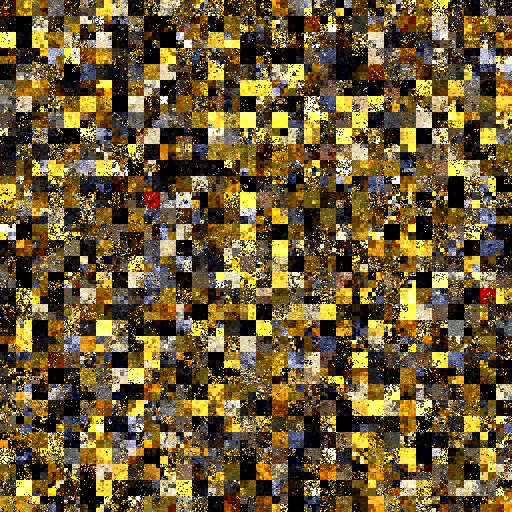
\includegraphics[height=\height]{assets/\clogdirname/plas/unsorted_colors.png} \&
        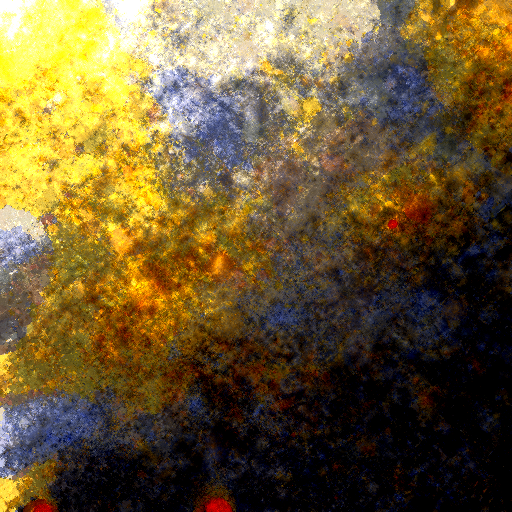
\includegraphics[height=\height]{assets/\clogdirname/plas/sorted_colors.png} \\
      };
      \node[above=0.4em of pictures-1-1.north, anchor=base] {Without PLAS};
      \node[above=0.4em of pictures-1-2.north, anchor=base] {With PLAS};
    \end{tikzpicture}
  }
}
\begin{figure}[t]
  \centering
  % \includegraphics[width=\linewidth, height=5em]{example-image-a}
  \plasfig
  \caption{\textbf{Effect of using PLAS~\cite{morgenstern2024compact} --}
    We demonstrate the effect of sorting by visualizing the decoded Gaussian
    colors in the UV map, for the \texttt{lego} sequence from the NeRF
    Synthetic~\cite{mildenhall2020nerf} dataset.
    After sorting, the UV map has smoother color transitions, confirming the
    successful spatial clustering of similar Gaussians.
  }
  \label{fig:clog-effect-of-plas}
\end{figure}

    \paragraph{Sorting.}
      After our 2D representation is trained, as mentioned in
      \cref{sec:clog-pipeline}, we downsample it to generate 2D maps for lower
      LoDs.
      This process requires neighboring features to exhibit similarity.
      To achieve this, we apply the PLAS
      algorithm~\cite{morgenstern2024compact} to latents $\cloglatents$.
      % Since, we effectively treat our 2D representation as an image and the
      % results of Stage I is unordered, to allow $\modulator$ to reuse
      % frequency dependency across different `pixels'. 
      Notably, we perform this sorting only \emph{once} at the end of Stage-I
      training, unlike in ~\cite{morgenstern2024compact} who apply it multiple
      times during training, which increases computational overhead.
      % Please note, that we apply PLAS once while
      % Morgenstern~\etal~\cite{morgenstern2024compact} uses PLAS multiple
      % times during training, slowing the process overall. 
      \cref{fig:clog-effect-of-plas} demonstrates PLAS's impact on the feature space by visualizing decoded Gaussian colors $\colors$ at their corresponding pixel locations.
      The post-sorting visualization reveals smooth color transitions,
      indicating successful spatial coherence of similar features.

      % mic: 40 drums: 0

% scan37: 6 scan114: 6 SCAN97: 0

% 20220412--1326--BGR645: 8 20220809--1034--BJM420: 3
\newcommand{\img}[5]{
  \includegraphics[height=\height]{assets/\clogdirname/qualitative/#1_#2_#3_#4_#5.png}
}

\newcommand{\clogqualitativefig}{
  \def\height{64bp}
  \tikzsetnextfilename{level_of_details}
  \resizebox{\linewidth}{!}{
    \begin{tikzpicture}[
        >=stealth',
        overlay/.style={
            anchor=south west,
            draw=black,
            rectangle,
            line width=0pt,
            outer sep=0,
            inner sep=0,
          },
      ]
      \matrix[
        matrix of nodes,
        column sep=-3pt,
        row sep=-0.1pt,
        ampersand replacement=\&,
        inner sep=0,
        outer sep=0
      ] (gts) {
        % \img{gt}{blender}{mic}{0040}{1.0} \\
        \img{gt}{blender}{drums}{0000}{1.0} \\
        \img{gt}{blender}{chair}{0040}{1.0} \\
        % \img{gt}{dtu}{scan37}{0006}{1.0} \\
        \img{gt}{dtu}{scan114}{0006}{1.0}   \\
        \img{gt}{dtu}{scan97}{0000}{1.0}    \\
        % \img{gt}{ava}{20220412--1326--BGR645}{0008}{1.0} \\
        % \img{gt}{ava}{20220809--1034--BJM420}{0003}{1.0} \\
      };
      \node[above=0em of gts-1-1.north] {Ground Truth};

      \matrix[
        right=1em of gts,
        matrix of nodes,
        column sep=-3pt,
        row sep=-0.1pt,
        ampersand replacement=\&,
        inner sep=0,
        outer sep=0
      ] (lvl1) {
        % \img{flod}{blender}{mic}{0040}{2} \&
        % \img{ours}{blender}{mic}{0040}{0.1} \\
        \img{flod}{blender}{drums}{0000}{2} \&
        \img{ours}{blender}{drums}{0000}{0.1} \\
        \img{flod}{blender}{chair}{0040}{2} \&
        \img{ours}{blender}{chair}{0040}{0.1} \\
        % \img{flod}{dtu}{scan37}{0006}{2} \&
        % \img{ours}{dtu}{scan37}{0006}{0.1} \\
        \img{flod}{dtu}{scan114}{0006}{2} \&
        \img{ours}{dtu}{scan114}{0006}{0.1}   \\
        \img{flod}{dtu}{scan97}{0000}{2} \&
        \img{ours}{dtu}{scan97}{0000}{0.1}    \\
        % \img{flod}{ava}{20220412--1326--BGR645}{0008}{2} \&
        % \img{ours}{ava}{20220412--1326--BGR645}{0008}{0.1} \\
        % \img{flod}{ava}{20220809--1034--BJM420}{0003}{2} \&
        % \img{ours}{ava}{20220809--1034--BJM420}{0003}{0.1} \\
      };

      \node[above=0em of lvl1-1-1.north] {FLoD};
      \node[above=0em of lvl1-1-2.north] {\textbf{Ours}};

      \matrix[
        right=1em of lvl1,
        matrix of nodes,
        column sep=-3pt,
        row sep=-0.1pt,
        ampersand replacement=\&,
        inner sep=0,
        outer sep=0
      ] (lvl3) {
        % \img{flod}{blender}{mic}{0040}{5} \&
        % \img{ours}{blender}{mic}{0040}{1.0} \\
        \img{flod}{blender}{drums}{0000}{3} \&
        \img{ours}{blender}{drums}{0000}{0.5} \\
        \img{flod}{blender}{chair}{0040}{3} \&
        \img{ours}{blender}{chair}{0040}{0.5} \\
        % \img{flod}{dtu}{scan37}{0006}{5} \&
        % \img{ours}{dtu}{scan37}{0006}{1.0} \\
        \img{flod}{dtu}{scan114}{0006}{3} \&
        \img{ours}{dtu}{scan114}{0006}{0.5}   \\
        \img{flod}{dtu}{scan97}{0000}{3} \&
        \img{ours}{dtu}{scan97}{0000}{0.5}    \\
        % \img{flod}{ava}{20220412--1326--BGR645}{0008}{3} \&
        % \img{ours}{ava}{20220412--1326--BGR645}{0008}{0.5} \\
        % \img{flod}{ava}{20220809--1034--BJM420}{0003}{3} \&
        % \img{ours}{ava}{20220809--1034--BJM420}{0003}{0.5} \\
      };

      \node[above=0em of lvl3-1-1.north] {FLoD};
      \node[above=0em of lvl3-1-2.north] {\textbf{Ours}};

      \matrix[
        right=1em of lvl3,
        matrix of nodes,
        column sep=-3pt,
        row sep=-0.1pt,
        ampersand replacement=\&,
        inner sep=0,
        outer sep=0
      ] (lvl5) {
        % \img{flod}{blender}{mic}{0040}{5} \&
        % \img{ours}{blender}{mic}{0040}{1.0} \\
        \img{flod}{blender}{drums}{0000}{5} \&
        \img{ours}{blender}{drums}{0000}{1.0} \\
        \img{flod}{blender}{chair}{0040}{5} \&
        \img{ours}{blender}{chair}{0040}{1.0} \\
        % \img{flod}{dtu}{scan37}{0006}{5} \&
        % \img{ours}{dtu}{scan37}{0006}{1.0} \\
        \img{flod}{dtu}{scan114}{0006}{5} \&
        \img{ours}{dtu}{scan114}{0006}{1.0}   \\
        \img{flod}{dtu}{scan97}{0000}{5} \&
        \img{ours}{dtu}{scan97}{0000}{1.0}    \\
        % \img{flod}{ava}{20220412--1326--BGR645}{0008}{5} \&
        % \img{ours}{ava}{20220412--1326--BGR645}{0008}{1.0} \\
        % \img{flod}{ava}{20220809--1034--BJM420}{0003}{5} \&
        % \img{ours}{ava}{20220809--1034--BJM420}{0003}{1.0} \\
      };

      \node[above=0em of lvl5-1-1.north] {FLoD};
      \node[above=0em of lvl5-1-2.north] {\textbf{Ours}};
    \end{tikzpicture}
  }
}

\begin{figure}
  \centering
  \clogqualitativefig
  \caption{
    \textbf{Qualitative highlight (varying levels of detail) --}
    We provide example renderings for various levels of detail, denoted by the
    number of Gaussians used.
    As shown, our method is able to provide high-quality reconstructions at
    various levels, and provides a better tradeoff than
    FLoD~\cite{seo2024flod}.
    We showcase the results for $\lod{\in}\{0.1, 0.5, 1.0\}$ for our method,
    and $\text{LoD}{=}\{2,3,5\}$ for FLoD to roughly match the number of
    Gaussians.
  }
  \label{fig:clog-level-of-details}
\end{figure}
  \subsection{Stage II -- Training the Modulator}
    % \paragraph{Stage II -- Training the Modulator $\modulator$} 

    With the highest-resolution UV map trained, we then downsample it to a
    given LoD $\lod$.
    % We then introduce a model that adapts pre-trained Gaussian parameters
    % $\gaussianset$ to a given LoD $\lod$.
    We use $\lod$ to first downsample our latents $\cloglatents$ and learned 3D coordinates $\threedcoords$ to the given resolution as:
    \begin{equation}
      \begin{aligned}
        \down{\cloglatents}  & = \downsample(\cloglatents, \lod),  \\
        \down{\threedcoords} & = \downsample(\threedcoords, \lod),
      \end{aligned}
    \end{equation}
    producing attributes $\down{\cloglatents},\down{\threedcoords} \in \real^{(\down{W} \times \down{H}) \times D}$ where:
    \begin{equation}
      \down{\width} = \floor{\width \cdot \lod}\quad \down{\height} = \floor{\height \cdot \lod}.
    \end{equation}
    From here on, we denote Gaussian attributes decoded from
    $\down{\cloglatent} \in \down{\cloglatents}$ as
    $\{\down{\mean},\down{\quat},\down{\scales},\down{\opacity},\down{\colors}\}$,
    where we drop the $i$-th index for brevity, and the resulting number of
    Gaussians is denoted as $\down{\width} \times \down{\height} =
    \down{\numgaussians}$

Since using $\lod < 1$ produces
    a smaller number of Gaussians than those contained in the entire set
    ($\down{\numgaussians} < \numgaussians$), the Gaussian parameters
    $\down{\cloglatents}$ need to be refined to compensate for missing
    Gaussians.
    % clarity.
    We introduce a parametrized latent modulator $\modulator$ with parameters
    $\modulatorparams$, conditioned on the level of detail $\lod$ that
    produces modulation vectors $\offset, \scale\in\real^\latentdim$.
    A single Gaussian descriptor $\cloglatent$ is modulated then as:
    \begin{align}
      \label{eq:clog-modulating}
      \offset(\cloglatent), \scale(\cloglatent) & = \modulator(\down{\cloglatent}, \lod\:;\: \modulatorparams )             \\
      \modulated{\cloglatent}                   & = \sigmoid(\scale(\cloglatent)) \odot \cloglatent + \offset(\cloglatent),
    \end{align}
    where $\sigmoid(\cdot)$ is a sigmoid activation function.
    Inspired by Continuous Upsampling Filters~\cite{vasconcelos2023cuf}, we
    implement $\modulator$ as an MLP that takes a latent $\cloglatent$
    concatenated with its corresponding 2D coordinate $\twodcoords{\in}[0,
    1]^2$ and the LoD value $\lod$.
    We additionally pass $\twodcoords$ and $\lod$ through a positional
    embedding function $\positionalemb(\cdot)$~defined as in traditional NeRF
    approaches~\cite{mildenhall2020nerf}.
    Overall, our $\modulator$ has the following form:
    \begin{equation}
      \label{eq:clog-modulator}
      \modulator(\cloglatent, \lod\:;\:\modulatorparams) = \mlp(\cloglatent, \positionalemb(\twodcoords), \positionalemb(\lod) \:;\:\modulatorparams).
    \end{equation}

    We optimize $\modulatorparams$ by minimizing the reconstruction objective (as in~\cref{eq:clog-first-stage-objective}) and corresponding regularization terms:
    \begin{equation}
      \argmin_{\modulatorparams} \loss{rec}^\modulator(\cloglatents, \networkparams, \modulatorparams)  + \regularizer^\modulator(\cloglatents, \modulatorparams),
    \end{equation}
    where $\regularizer^\modulator$ is the modulator-specific regularization term where we minimize $\left\|1 - \offset(\cloglatent)\right\|_2^2$ and $\left\|\scale(\cloglatent)\right\|_2^2$, such that the modulator is encouraged to perform an identity transform.

  \subsection{Implementation details}
    For the latents $\cloglatents$, we use the descriptor dimension
    $\latentdim{=}16{\times}6$ meaning that each attribute consists of its own
    descriptor.
    We represent colors~$\colors$ as Spherical Harmonics of the second degree.
    For the decoding MLPs in \cref{eq:clog-decoders}, we use two layers, each
    with 64 neurons.
    For the modulator~$\modulator$ we use an MLP with six layers, each with
    256 neurons.
    We encode $\twodcoords$ using the hash grid from
    InstantNGP~\cite{mueller2022instant}.
    We use a hashgrid size of $2^{19}$ elements which holds 16 levels of
    2-dimensional feature vectors.
    For the scale component we use frequency
    encodings~\cite{mildenhall2020nerf}---we use 8 frequencies, increasing by
    a power of 2 starting from 1.
    % We refer the reader to our implementation for values less impactful
    % hyperparameters. 
    Regarding hyperparemters, we set them identically for all experiments.
    We use a regularization strength of $10^{-2}$ for
    $\|\opacity_i(\cloglatent_i)\|_1$, $10^{-4}$ for
    $\|\scales_i(\cloglatent_i)\|_2^2$, $10^{-2}$ for both $\left\|1 -
    \offset(\cloglatent)\right\|_2^2$ and
    $\left\|\scale(\cloglatent)\right\|_2^2$, all set empirically.
    % We \todo{provide more details} in~\supplementary{}.

    We initialize our 3D coordinates from a quasi-random Halton sequence from
    the $[-1, 1]^3$ range.
    We train the representation starting with a $32^2$ grid.
    We first warmup the training for 500 steps, then progressively grow it by
    doubling its size every 2000 steps.
    We train both stages for $10^5$ steps so the training takes $2 \times
    10^5$ steps in total.
    We implement our method using the
    \texttt{gsplat}~\cite{ye2024gsplatopensourcelibrarygaussian} library.
    % We will release our code upon acceptance.
